%-------------------------------------------------------------------------------
\chapter[Introduction]{Introduction to Gaia}
%-------------------------------------------------------------------------------

%-------------------------------------------------------------------------------
\section{Preliminaries}
%-------------------------------------------------------------------------------
\gaia{} is the open-source, sediment transport and bed evolution module of the \telemacsystem{}. This module can be used to model complex sediment and morphodynamics processes in coastal, rivers, lakes and estuaries, accounting for spatial and temporal variability of sediment size classes (uniform, graded or mixed), properties (cohesive and non-cohesive) and transport modes (suspended and bedload).

\gaia{}'s is based on the historical sediment transport module \sisyphe{}, where a large number of improvements, corrections and optimizations have been implemented.
Thanks to its unified framework, \gaia{} efficiently manages different sediment classes, sand-mud mixtures, etc. for both 2D and 3D cases.

Although transparent for the user, suspended sediment transport processes are dealt by the hydrodynamic modules (\telemac{2D} or \telemac{3D}), while near-bed, bedload and stratigraphic processes process are lead by \gaia{}. This allows a clearer treatment of sedimentary processes that happen in the water column, in the bottom and in the interface water-bottom. Furthermore, within the new informatic structure, is performed in terms of mass instead of volume, which minimizes roundoff errors. 

Sediment transport processes are grouped as bedload, suspended load or total load,
with an extensive library of predictors for sediment transport carrying capacity. It is applicable to non-cohesive sediments that can be uniform (single-sized) or non-uniform
(graded), cohesive sediments, as well as sand-mud mixtures. Furthermore, vertical stratification of sediments can be considered via multi-layer model.

A number of physically-based processes are incorporated into \gaia{}, such as the influence of
secondary currents to precisely capture the complex flow field induced by channel curvature, the
effect of bed slope associated with the influence of gravity, bed roughness predictors, and areas of
non-erodible bed, among others.

%For currents only, \gaia{} can be coupled to the depth-averaged shallow water module
%\telemac{2D} or to the three-dimensional Reynolds-averaged Navier-Stokes module \telemac{3D}.
%To account for the effect of waves or combined waves and currents, \gaia can be internally coupled
%to the waves module \tomawac{}.

\gaia{} can easily be expanded and customized to particular requirements by modifying friendly,
easy to read fortran files. An overview of different applications of \gaia{} can be consulted in the yearly-published Telemac-Mascaret User Conference proceedings, freely available at the website \texttt{www.opentelemac.org}.

%\begin{figure}[H]%
%\begin{center}
%
%\hfil
%
%\subfloat[Bar formation and propagation in straight channels: simulations by \gaia{} coupled to \telemac{2D} (based on the works by Defina~\cite{Defina2003} and Crosato et al.~\cite{Crosato2011})]{
%
%  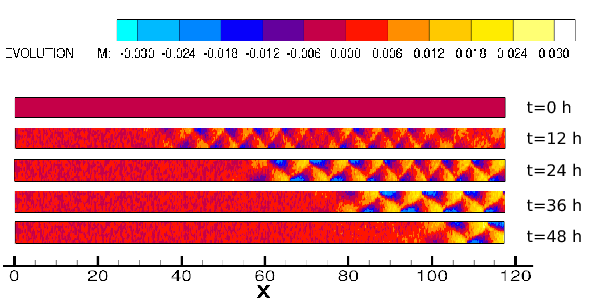
\includegraphics[width=0.5\textwidth]{./graphics/T2d+Sis_Lanzoni_random_10mm_Planimetric.png}
%
%}
%
%\hfil
%
%\subfloat[Point bars in large-amplitude meanders: simulations by \gaia{} coupled to \telemac{2D} and \telemac{3D} (based on the experiences by Whiting and Dietrich~\cite{Whiting1993a, Whiting1993b}.]{
%
%  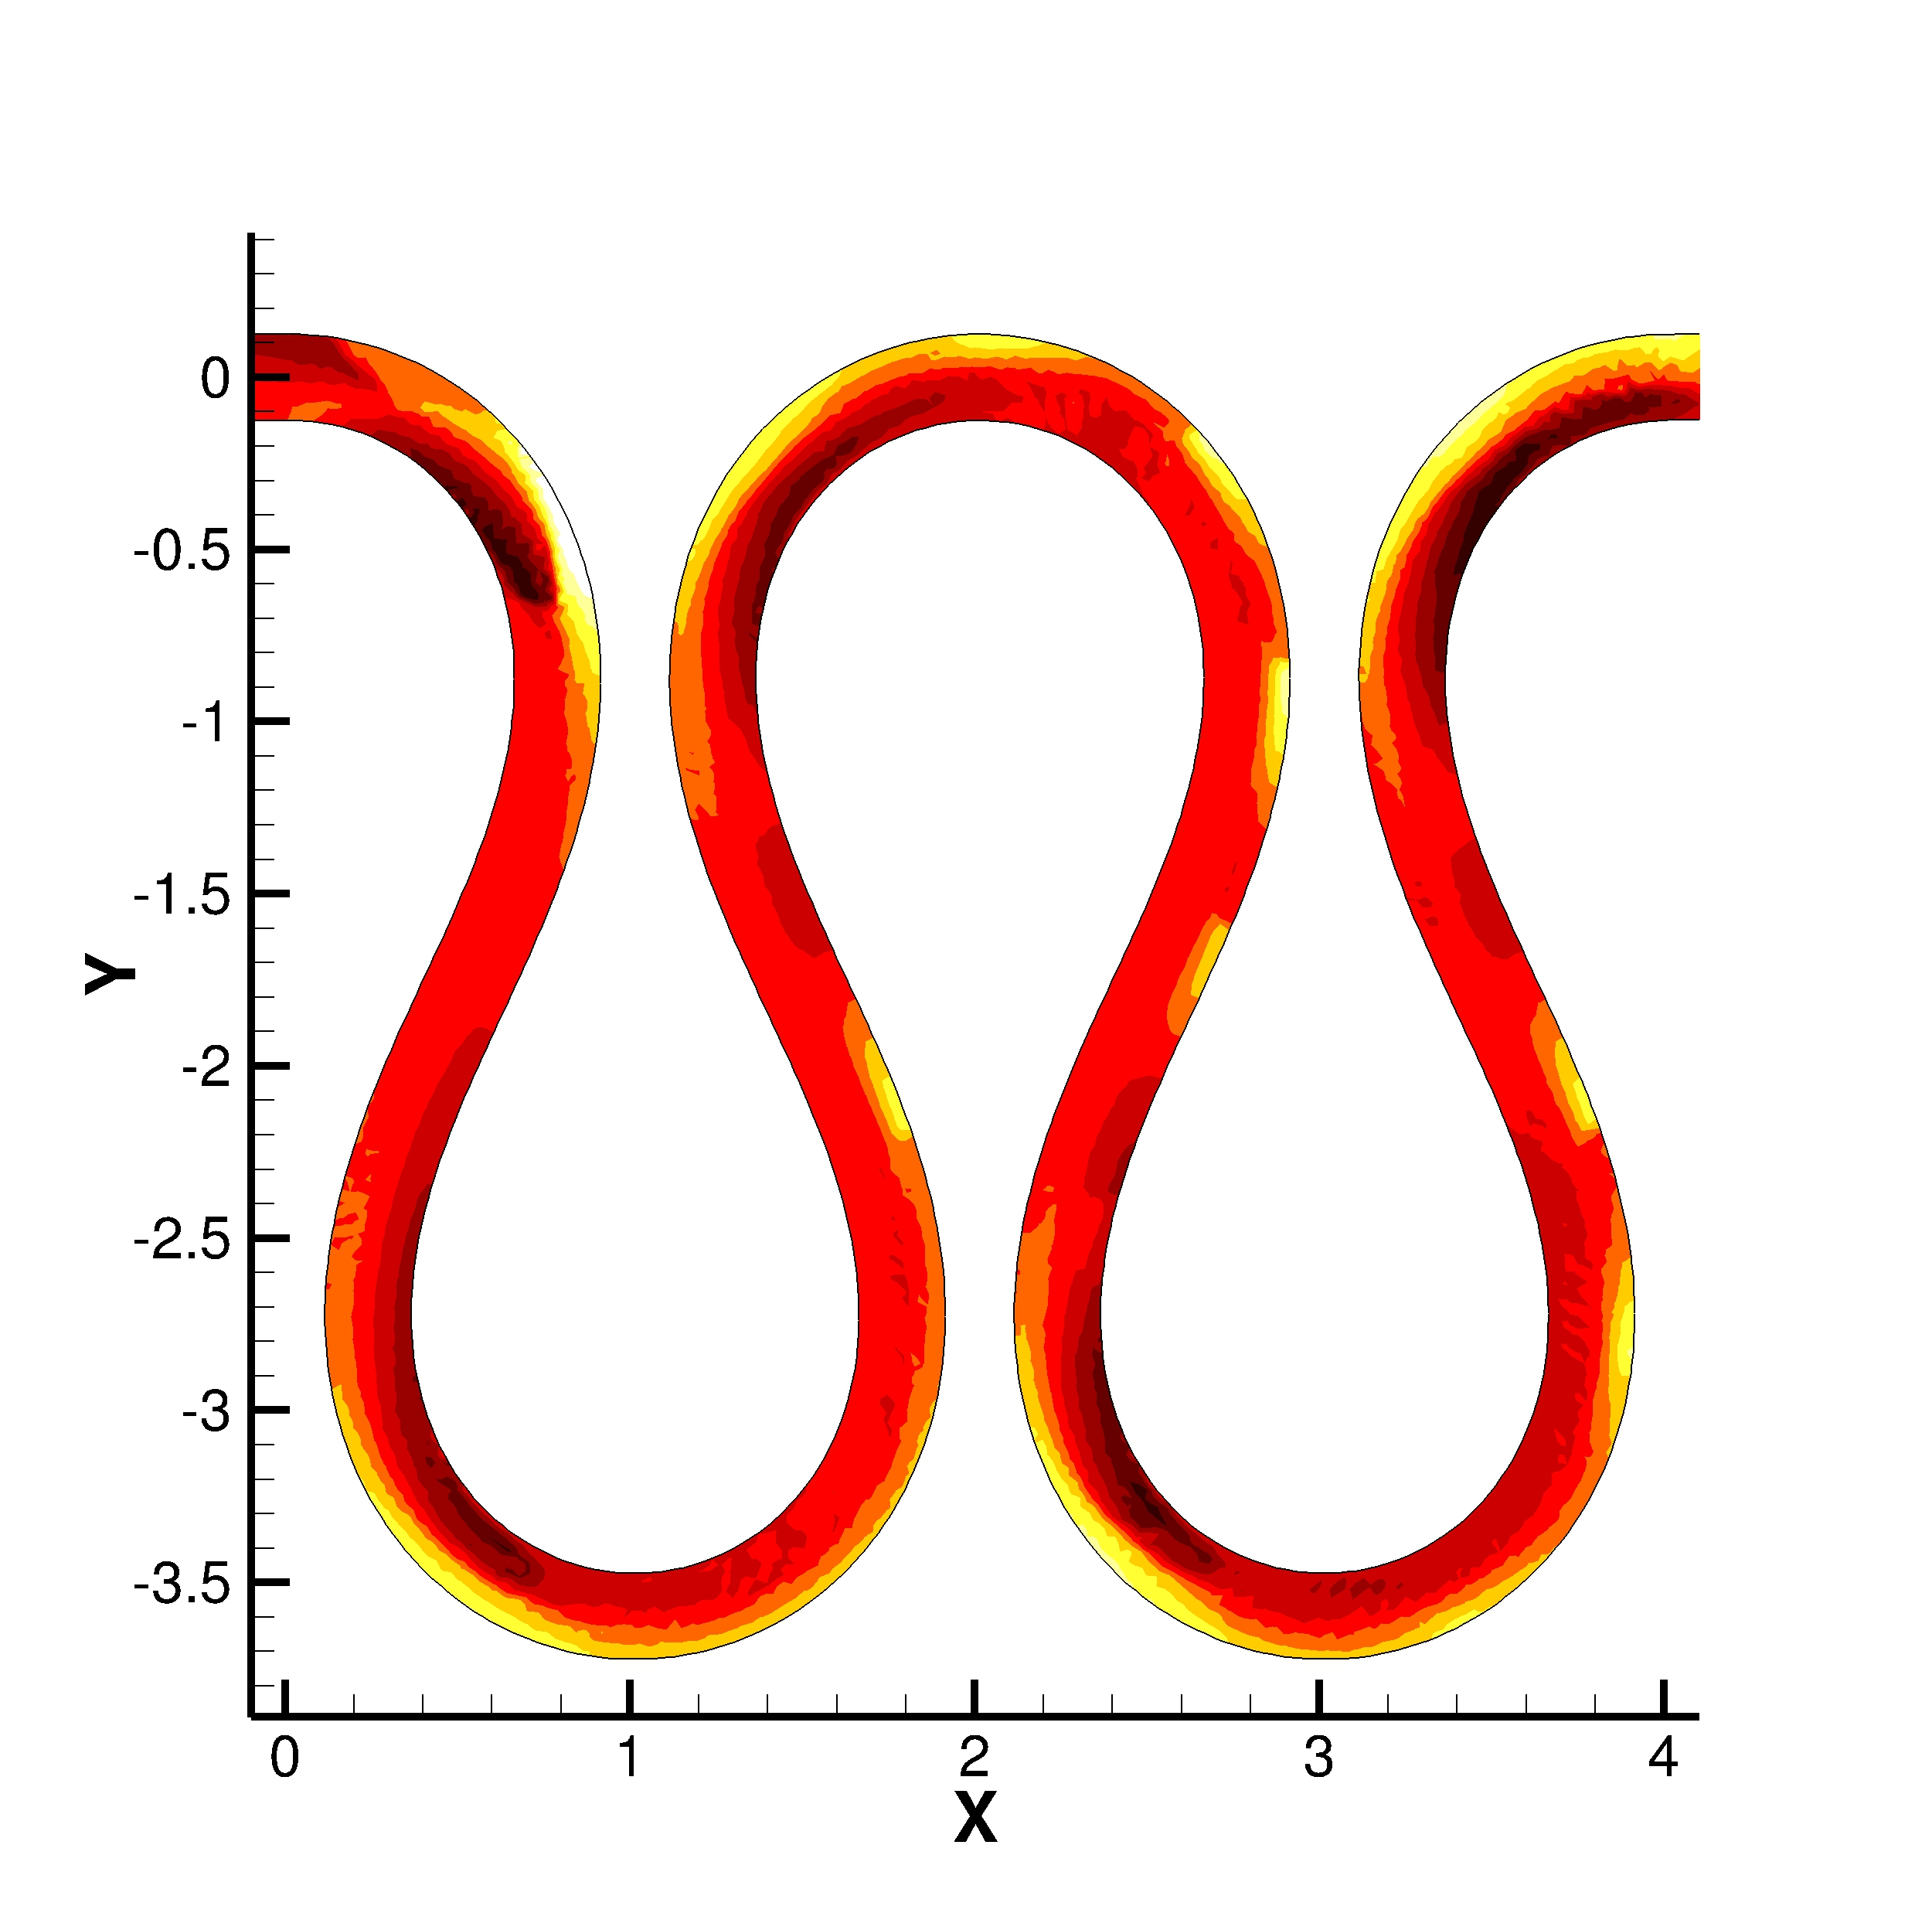
\includegraphics[width=0.35\textwidth]{./graphics/2D.jpg}
%
%}

%
%\hfil
%\mbox{}
%\end{center}
%\caption
%[Examples of morphodynamics modelling]
%{Examples of morphodynamics modelling of bar formation and propagation in straight and curved channels. See also proceedings of the Telemac-Mascaret User Conference 2013.}
%\label{fig:ExampleMultipleImages}
%\end{figure}

%-------------------------------------------------------------------------------
\subsection{Morphodynamic modelling}
%-------------------------------------------------------------------------------
The prediction of topography changes and sediment discharges can be performed by integrating several modules. It is a {\bf multi--scale problem}, with different physical mechanisms acting according to their space and time response. In summary, the relevant mechanisms that drives morphological changes are:
\begin{itemize}
         \item {\bf Hydrodynamics}, with conservative laws of mass and momentum
         \item {\bf Sediment transport}, with predictors for sediment transport capacity
         \item {\bf Bed evolution}, with conservative law for sediment mass
\end{itemize}
\noindent
Such a modelling system is often referred to as a \emph{morphodynamic model} and is the one adopted in the \telemacsystem{}.

\noindent
From the literature, the mechanisms of transport are mainly classified as:
\begin{itemize}
\item \textcolor{black}{\bf bedload:} with a variety of sediment transport formulations
\item \textcolor{black}{\bf suspended load:} with the solution of the advection-diffusion equation (ADE) plus closures for erosion and deposition fluxes, equilibrium concentration
\item \textcolor{black}{\bf bed evolution:} with the solution of the sediment mass conservation equation or \textit{Exner equation}.
\end{itemize}

\noindent
Different types of sediment can be classified as:
\begin{itemize}
\item \textcolor{black}{\bf non-cohesive:} equilibrium formulas
\item \textcolor{black}{\bf cohesive:} erosion and deposition laws, consolidation models
\item \textcolor{black}{\bf mixed-size sediments:} moderately/poorly sorted sediment distribution, sand-gravel and sand-mud mixtures
\end{itemize}
\noindent


%-------------------------------------------------------------------------------
\subsection{Choice of hydrodynamic modelling for morphodynamic models}
%-------------------------------------------------------------------------------
The choice of appropriate model equations for flow and sediment transport
will depend upon the scales of interest.

At the scale of ripples, the mechanics of sediment transport could be coupled with the
Reynolds--averaged Navier Stokes equations (NS) to describe the phenomenon.
At large scales, however, the shallow water equations (SWE) are known to
capture quite accurately the salient features --in an average sense-- of
open channel flows. The SWE are derived by simplifying the hydrodynamics in the vertical
direction instead of using the full three--dimensional NS or Euler
equations.

As such, the SWE are obtained by assuming a hydrostatic pressure
distribution and a uniform velocity profile across the water layer,
resulting in a two--dimensional problem where the primary variables are the
vertical averages of the horizontal fluid velocities and the fluid depth.

This simplification enhances the speed of computations and
facilitates further analytical approaches. In brief, the SWE are often
used to model advection--dominated open channel flows, river and lake
hydrodynamics, floodplain flows, estuarine and coastal circulation as well
as long wave run-up and hydraulic bores, among
other problems of interest within the engineering community~\cite{Vreugdenhil:94}.

\gaia{} can be coupled with the SWE solver \telemac{2D} and the NS solver \telemac{3D} (see \S\ref{ch:3DBedloadTransport}).

%-------------------------------------------------------------------------------
\subsection{Coupling hydrodynamics to morphodynamics}
%-------------------------------------------------------------------------------
Morphological models can be run fully coupled~\cite{cao02} and decoupled~\cite{vriend87}. In a fully coupled model, sediment
transport and flow occur simultaneously, and thus, their respective
equations are coupled and should be solved simultaneously. Rapid morphological evolution processes due
to hyper-concentrated sediment--laden floods, and debris flow are typical
examples were the fully coupled approach must be employed~\cite{Frac02}.

In contrast, decoupled models are applicable when the typical time scale for river or sea bed adjustment
is much longer than the typical time scale for water flow. The approach used by \gaia{} follows the decoupled treatment, i.e., to alternate between the simulation of flow and bed evolution. This procedure, also known as \textit{asynchronous} solution, considers that the bottom is fixed when the flow variables are computed.

Hydrodynamic solution is therefore to solve the hydrodynamic continuity and momentum equations on a short time scale.
During this hydrodynamic step the bottom is freezed and the discretized sediment equation is subsequently solved separately.


\begin{figure}[H]%
\begin{center}
%
\hfil
%
\subfloat[currents only]{
  %
  \vspace{-1cm}
  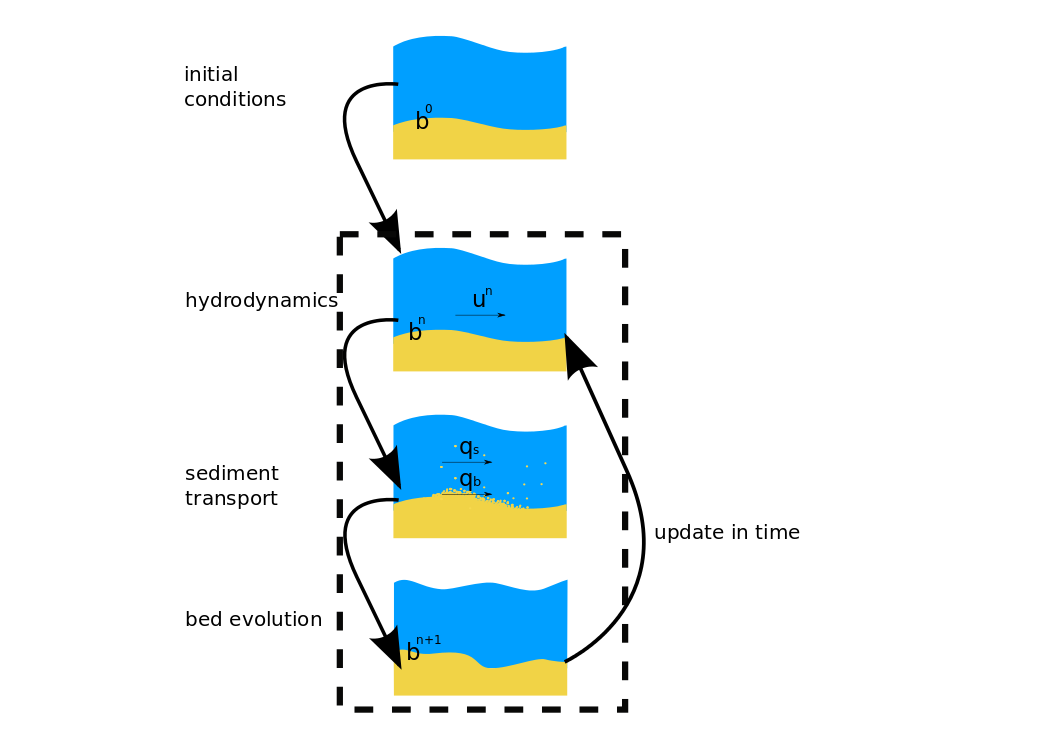
\includegraphics[width=0.55\textwidth]{./graphics/2waycoupling.png}
%
}
%
\hfil
%
\subfloat[currents $+$ waves]{
%
  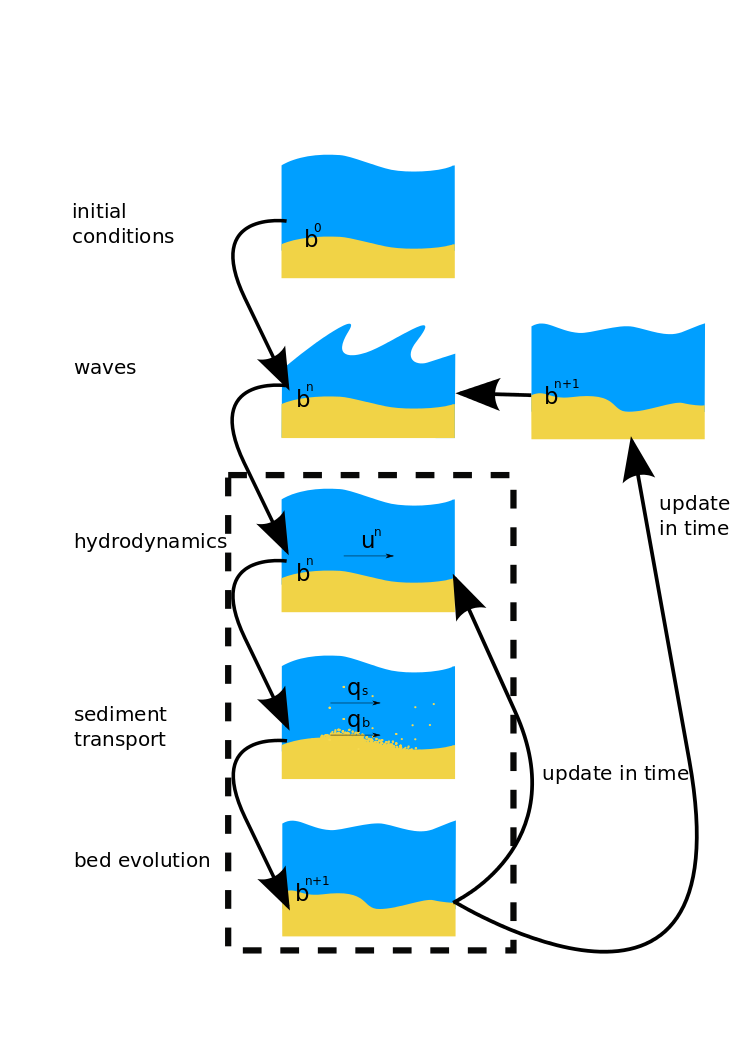
\includegraphics[width=0.4\textwidth]{./graphics/3waycoupling.png}
%
}
%
\hfil
\mbox{}
\end{center}
\caption
[Coupling strategies]
{Schematic coupling strategies for \gaia: (a) coupling morphodynamic and hydrodynamic, current only, (b) coupling morphodynamic and hydrodynamic including the effect of waves.}
\label{fig:CouplingStrategies}
\end{figure}

\pagebreak

%-------------------------------------------------------------------------------
\section{Gaia's structure}
%-------------------------------------------------------------------------------

%...............................................................................
\subsection{Coupling hydrodynamics and morphodynamics}
%...............................................................................
\gaia{} can be internally coupled with the hydrodynamic models \telemac{2D} or \telemac{3D}. In the \telemac{2D} or \telemac{3D} steering files, the following keywords need to be specified:
\begin{itemize}
\item \telkey{COUPLING WITH = 'GAIA'}
\item \telkey{GAIA STEERING FILE = '<name of the gaia steering file>'}
\end{itemize}
For a \textit{hotstart} from a fully developed hydrodynamic, the following information must be included in the \telemac{2D} or \telemac{3D} steering files:
\begin{itemize}
\item \telkey{COMPUTATION CONTINUED} (logical type, set to {\ttfamily = NO} by default)
\end{itemize}
The file name is provided with the keyword \telkey{PREVIOUS COMPUTATION FILE}. Optionally, \telkey{INITIAL TIME SET TO ZERO} (logical type, set to {\ttfamily = NO} by default).

The time step used for morphodynamic computation is the same used for hydrdynamics. It is specified in the \telemac{2D} or \telemac{3D} steering file. For suspended load, the advection-diffusion equation obeys the same Courant number criteria on the time step than the hydrodynamics, and therefore needs to be solved at each time-step. Typically the morphodynamic scale induced by bed load is much smaller, than the hydrodynamic scale. This leads to very small bed level changes in a hydrodynamic time step. The use of a coupling period $>1$ is  very useful in this case. It allows the bed load transport rates and resulting bed evolution not to be re-calculated at every time step.

%...............................................................................
\subsection{Mixed and graded sediment}
%...............................................................................
TODO

%...............................................................................
\subsection{Equivalence between \gaia{} and \sisyphe{}}
%...............................................................................
We refer the reader to Appendix~\ref{appen:1} for an overview of the equivalence between keywords of \sisyphe{} and \gaia{}. Mandatory keywords to include in \gaia{}'s steering files are:
\begin{itemize}
\item \telkey{TYPE OF SEDIMENT}
\item \telkey{BED LOAD FOR ALL SANDS}
\item \telkey{SUSPENSION FOR ALL SANDS}
\item \telkey{BED-LOAD TRANSPORT FORMULA FOR ALL SANDS}
%\item \telkey{SETTLING VELOCITIES}
%\item \telkey{SHIELDS PARAMETER}
%\item \telkey{SEDIMENT DENSITY}
\end{itemize}
%\pagebreak

